\section{Visual Grounding, Identity, and Uncertainty}\label{app:G}
\subsection{What the localization diagnostic measures}
The N2 task supplies a point at which to inspect an object and an optional class hint. Models then provide an image box and a physical-entity assignment. The reference boxes support a given-point localization diagnostic. They do not turn the experiment into automatic object detection: neither discovery recall over an entire drawing nor recovery of every room, opening, and stair is measured.

The primary overlap threshold is IoU $\geq0.25$. The criterion is relatively permissive and is reported with mean IoU and missing/unevaluable records. It measures approximate 2D extent around a specified target. It cannot by itself validate metric 3D placement, a host wall, a floor assignment, or cross-view physical identity. A model can put a reasonable box around an object while assigning it to the wrong instance.

\begin{table}[htbp]\centering
\begin{tabular}{llrrr}\toprule Input & Route & IoU gate & Mean IoU & Ref. NE\\\midrule
N2 & A & 446/656 & .491 & 16\\
N2 & B & 440/656 & .489 & 16\\
CS1 & A & 49/88 & .320 & 0\\
CS1 & B & 40/88 & .269 & 0\\\bottomrule
\end{tabular}
\caption{GPT localization, pooling the eight configurations. Ref. NE is reference-not-evaluable and is outside the listed IoU denominator. These are approximate image boxes at supplied points.}\label{tab:G-grounding}
\end{table}

Relation assistance does not improve these aggregate localization measures. N2 A/B mean IoU is almost unchanged, while CS1 B is lower. Correct relation values therefore do not substitute for locating the right image extent. The association is descriptive: A and B are independent generations, and the experiment does not isolate every possible localization mechanism.

\subsection{Observations, instances, and repeated labels}
An observation is a visible occurrence on a drawing; an entity is the physical instance that an observation may denote. Multiple observations can map to one entity. Two different windows can share a printed type code. A staircase assembly and one of its runs can overlap in an image without being the same semantic unit.

The executable reader's identity predicate compares submitted observation bindings. If two requested observations explicitly name the same entity, it reads SAME; unresolved bindings yield UNKNOWN. This is an inspectable output claim, not independent proof that the entity truly corresponds to the source building. Image-based qualification is still needed. The benchmark therefore reports identity readouts alongside grounding rather than treating either as a complete substitute for the other.

Figure~\ref{fig:G-identity} provides a source-linked identity example from Idaho City Schoolhouse. Its two crops correspond to O02 and O03 on different assigned pages. The frozen Q08 reference is TRUE. The audit links each crop to a public page and preserves its parent image hash. These human-review crops were not additional inputs during the model trials.

\begin{figure}[htbp]\centering
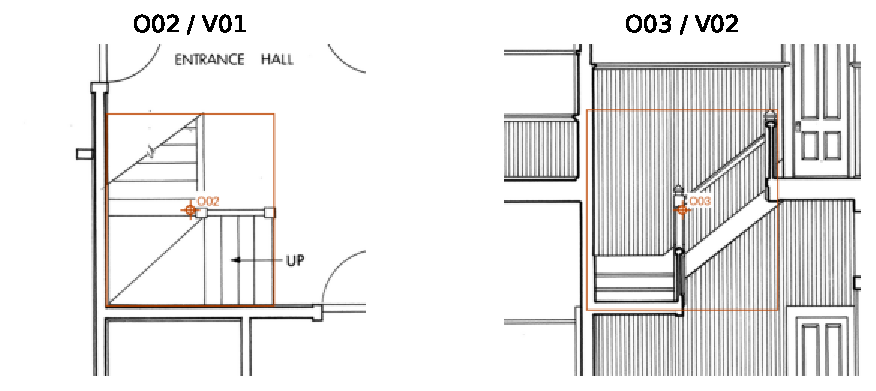
\includegraphics[width=.95\linewidth]{figures/identity_evidence.pdf}
\caption{Two drawing observations of the internal staircase in C03 (Q08). This is a reference-evidence panel, not a model detection. Image crops are shown for inspection; the package retains the complete pages. A correct identity binding does not by itself certify that the generated staircase is free of slab intrusion.}\label{fig:G-identity}
\end{figure}

\subsection{UNKNOWN as a supported result}
The unique unresolved identity concerns B04's cross-era observations. v1 returns the appropriate unresolved result in 18 of 24 allocations; N2 does so in only two of 24. The other 22 N2 outputs make unsupported definite assignments. Because the evidence does not establish a unique identity, these are failures of calibrated evidence use, not 22 independently proven physical mismatches.

Qwen R and A make definite SAME claims for this obligation. Its B task is missing because of the API service failure. These are two unsupported-certainty results and one unavailable result. The service failure is not reclassified as an identity decision. With only one uncertainty-bearing relation, the experiment cannot estimate a general calibration curve or uncertainty-detection accuracy across architecture.

\subsection{Source names and binding reliability}
A source identifier links a box or observation to its input image. An unrecognized alias can make the output hard to score even if the box is visually plausible. Appendix~\ref{app:F} reports the Qwen alias diagnostic separately. The same discipline applies to missing observations, duplicated entity IDs, and semantic target names: a convenient guessed mapping must not silently become reference truth.

The released records retain requested anchor IDs, source IDs, observation boxes, and entity bindings. This allows an auditor to distinguish at least four failures: no box at the requested point, a wrong extent, a source-ID mismatch, and a wrong physical binding despite a plausible box. The current aggregate score alone does not count all of these mechanisms independently; detailed cases must be inspected rather than inferred from the mean IoU.

The next grounding experiment should add more independently qualified same/different/unknown pairs and separate them from query wording. It should also test automatic candidate discovery without supplied points. Those are future measurements, not capabilities established by the current point-anchored record.
